%\documentclass[10pt]{beamer}
%\usepackage{xeCJK}
  \documentclass[handout,10pt]{beamer}
%\usepackage[orientation=landscape,size=custom,width=16,height=14,scale=0.5,debug]{beamerposter}
 % 1. packages

 % ----------- fonts and symbles ---------
\usepackage{amsmath,amssymb,amsfonts,amsthm}
%\usepackage{CJK}
\usepackage{dsfont}
\usepackage{mathrsfs}
\usepackage{eucal} % for \mathcal

%\renewcommand{\rmdefault}{ptm}


%\usepackage{fontspec}
%\newfontfamily\monaco{Monaco}

%\usepackage{mathbbold} %,bbold

 \usepackage{textcomp} % for \textnormal{\textperthousand}
% -----------------





%\usepackage{slashbox}
%\usepackage[margin=2.2cm]{geometry} % |geometry| package clash with |booktabs| package
%\usepackage{cases}
% -------- tables -------
\usepackage{booktabs} % for \toprule, \bottomrule
\usepackage{tabularx}
\usepackage{multirow}
% --------- figures ---------
\usepackage{graphicx}
% ---------- algorithms -------
\usepackage{algorithm}
\usepackage{algorithmic}
%\usepackage{footnote}
    % |footnote| package occurs error:
    % Runaway argument?
    % \def \insertfootnotetext {\@@ }\def \insertfootnotemark {\@makefnmark \ETC.

\usepackage{listings}

\usepackage[linewidth=1pt]{mdframed} % for  mdframe environment




 \usepackage{color}
 \usepackage{xcolor}     %¸ßÁÁʹÓõÄÑÕÉ«

\usepackage{setspace}
%%\usepackage{type1cm}
\usepackage{adjustbox} % for \adjustbox

\usepackage{accsupp}
\newcommand{\emptyaccsupp}[1]{\BeginAccSupp{ActualText={}}#1\EndAccSupp{}}




%%   figures and tables
\graphicspath{{figure/}}


% 2. new commands

% 2.0 common commands
%\newcommand{\bc}{\begin{center}}
%\newcommand{\ec}{\end{center}}
%\newcommand{\ba}{\begin{array}}
%\newcommand{\ea}{\end{array}}
%\newcommand{\be}{\begin{equation}}
%\newcommand{\ee}{\end{equation}}

% 2.1 colors
\definecolor{dgrey}{rgb}{0.30,0.30,0.30}
\definecolor{lred}{rgb}{0.50,0.00,0.50}
\definecolor{lblue}{rgb}{0.8,0.8,1}
\definecolor{dred}{rgb}{0.6,0,0}
\definecolor{dblue}{rgb}{0,0,0.5}
\definecolor{dgrey}{rgb}{0.35,0.35,0.35}
\definecolor{rred}{rgb}{0.9,0,0}
\definecolor{mylblue}{rgb}{0.3,0.2, 0.8}

\definecolor{commentcolor}{RGB}{85,139,78}
\definecolor{stringcolor}{RGB}{206,145,108}
\definecolor{keywordcolor}{RGB}{34,34,250}
\definecolor{backcolor}{RGB}{220,220,220}

\newcommand{\blue}[1]{{\color{blue}#1}}
\newcommand{\dblue}[1]{{\color{dblue}#1} }
\newcommand{\red}[1]{{\color{red}#1}}
\newcommand{\dred}[1]{{\color{dred}#1}}
\newcommand{\cyan}[1]{{\color{cyan}#1}}
\newcommand{\bfblue}[1]{\textbf{\color{dblue}#1} }
\newcommand{\bfred}[1]{\textbf{\color{dred}#1} }
\newcommand{\green}[1]{{\color{green}#1}}
%\newcommand{\alert}[1]{{\color{red}#1}}
\newcommand{\black}[1]{{\color{black}#1}}
\newcommand{\light}[1]{{\color{blue}\textbf{#1}}}
\newcommand{\hot}[1]{{\color{dred}#1}}
 \newcommand{\highlight}[1]{ \textbf{\color{mylblue}#1}}
 \newcommand{\important}[1]{{\color{red}#1}} % for highlighting  some words

 \newcommand{\mystar}{\dred{$^{\clubsuit}$ }}
  \newcommand{\doublestar}{\dred{$^{\clubsuit\clubsuit}$ }}

\newcommand{\mynote}[1]{{\footnotesize \color{mylblue}#1}}

 \newcommand{\hint}[1]{{\small \color{mylblue}#1}}
\newcommand{\smallhint}[1]{{\small \color{dgrey}#1}}
\newcommand{\footnotehint}[1]{{\footnotesize \color{dgrey}#1}}
\newcommand{\tinyhint}[1]{{\tiny \color{dgrey}#1}}
\newcommand{\mytitle}[1]{\medskip{\large \textbf{\color{mylblue}#1}}}
\newcommand{\normaltitle}[1]{\medskip{ \textbf{\color{mylblue}#1}}}

%\newcommand{\head}[1]{\textbf{\large\color{blue}#1}}
%\newcommand{\heading}[1]{\textbf{\large\color{blue}#1}}

\newcommand{\myfbox}[2]{ \bigskip \begin{center} \fbox{\parbox{#1}{ #2  }} \end{center}\bigskip }

\newcommand{\myvar}[1]{}
%\newcommand{\mynote}[1]{#1}

% 2.2 mathematical symbols

\newcommand{\drightarrow}{\stackrel{d.}{\rightarrow}}
\newcommand{\prightarrow}{\stackrel{p.}{\rightarrow}}
\newcommand{\bernoulli}{\textnormal{Ber}}
\newcommand{\cov}{\mathsf{Cov}}
\newcommand{\corr}{\mathbf{Corr}}
\newcommand{\regret}{\textnormal{Regret}}
\newcommand{\conv}{\textnormal{conv}}
\newcommand{\dotdiv}{\stackrel{\centerdot}{-}}
\newcommand{\dom}{\textnormal{dom}}
\newcommand{\convergenceinprob}{\stackrel{P}{\rightarrow}}
\newcommand{\convergenceindist}{\rightsquigarrow}
\newcommand{\probability}{\mathbb{P}}
\newcommand{\expectation}{\mathbb{E}}
\newcommand{\epi}{\textnormal{epi}}
\newcommand{\variance}{\mathbb{V}}
\newcommand{\var}[1]{\mathbb{V}(#1)}
\newcommand{\covariance}{\mathsf{Cov}}
\newcommand{\empiricalrisk}[1]{\hat{R}(#1)}
\newcommand{\expectedrisk}[1]{R(#1)}
\newcommand{\mgf}[1]{\psi_{#1}(\lambda)}
\newcommand{\mgfexpansion}[1]{\expectation[e^{\lambda#1}]}
\newcommand{\mgfmultivariate}[1]{\expectation[e^{\lambda^\transpose#1}]}
\newcommand{\transpose}{{\mathsf{T}}}
\newcommand{\real}{\mathbb{R}}
\newcommand{\gaussian}[2]{\mathcal{N}(#1,#2)}
\newcommand{\subGaussian}[1]{\mathsf{subG}(#1)}
\newcommand{\indicator}[1]{\mathbb{I}[#1]}
\newcommand{\x}[1]{x^{(#1)}}
\newcommand{\y}[1]{y^{(#1)}}
\newcommand{\z}[1]{z^{(#1)}}
\newcommand{\feature}{x}
\newcommand{\response}{y}
\newcommand{\supofempiricalprocess}{\|\mathbb{P}_n-\mathbb{P}\|_{\decisionspace}}
\newcommand{\decisionspace}{\mathscr{F}}
\newcommand{\decisionfunction}{f}
\newcommand{\featurespace}{\mathcal{X}}
\newcommand{\classifierestimate}{\widehat{h}}
\newcommand{\classifiertrue}{h^\star}
\newcommand{\classifier}{h}
\newcommand{\hypothesisclass}{\mathcal{H}}
\newcommand{\dataset}{\mathcal{D}}
\newcommand{\defineas}{\stackrel{\textnormal{def}}{=}}
\newcommand{\rademachercomplexity}[1]{\mathsf{Rad}_n\left(#1\right)}
\newcommand{\loss}{\ell}
\newcommand{\composite}{\circ}
\newcommand{\convexhull}{\mathsf{conv}}
\newcommand{\norm}[2][2]{\|#2\|_{#1}}
\newcommand{\shatteringcoefficient}[2]{\mathcal{S}(#1,#2)}
\newcommand{\vcdimension}[1]{\mathsf{VC}\left(#1\right)}
\newcommand{\rank}{\mathsf{rank}}
\newcommand{\innerproduct}[2]{\left\langle #1, #2\right\rangle}
\newcommand{\modelparameter}{\theta}
\newcommand{\ball}[3][]{\mathcal{B}_{{#1}}\left(#2,#3\right)}
\newcommand{\metric}{d}
\newcommand{\coveringnumber}[4][]{N_{{#1}}\left(#2,#3,#4\right)}
\newcommand{\trace}{\textnormal{tr}}
\newcommand{\std}{\textnormal{std}}
\newcommand{\sgn}{\textnormal{sign}}
%\renewcommand{\span}{\textnormal{span}}

 % do not overwrite the existing command \span
 % as it leads to an error of
 %  "Missing # Inserted in Alignment Preamble" for ``align'' environment

\newcommand{\myspan}{\textnormal{span}}

%%%
\newcommand{\rightarrowd}{\stackrel{d}{\rightarrow}}
\newcommand{\rightarrowp}{\stackrel{p}{\rightarrow}}
\newcommand{\defeq}{ \stackrel{\textnormal{def}}{=}}
\newcommand{\proj}{ \textnormal{Proj}}
\newcommand{\dist}{\textnormal{dist}}

\newcommand{\argmax}{\textnormal{argmax}}
\newcommand{\argmin}{\textnormal{argmin}}
\newcommand{\subg}{\textnormal{subG}}


 \newcommand{\bba}{\mathbb{A}}
\newcommand{\bbb}{\mathbb{B}}
\newcommand{\bbc}{\mathbb{C}}
\newcommand{\bbd}{\mathbb{D}}
\newcommand{\bbe}{\mathbb{E}}
\newcommand{\bbf}{\mathbb{F}}
\newcommand{\bbg}{\mathbb{G}}
\newcommand{\bbh}{\mathbb{H}}
\newcommand{\bbi}{\mathbb{I}}
\newcommand{\bbj}{\mathbb{J}}
\newcommand{\bbk}{\mathbb{K}}
\newcommand{\bbl}{\mathbb{L}}
\newcommand{\bbm}{\mathbb{M}}
\newcommand{\bbn}{\mathbb{N}}
\newcommand{\bbo}{\mathbb{O}}
\newcommand{\bbp}{\mathbb{P}}
\newcommand{\bbq}{\mathbb{Q}}
\newcommand{\bbr}{\mathbb{R}}
\newcommand{\bbs}{\mathbb{S}}
\newcommand{\bbt}{\mathbb{T}}
\newcommand{\bbu}{\mathbb{U}}
\newcommand{\bbv}{\mathbb{V}}
\newcommand{\bbw}{\mathbb{W}}
\newcommand{\bbx}{\mathbb{X}}
\newcommand{\bby}{\mathbb{Y}}
\newcommand{\bbz}{\mathbb{Z}}

\newcommand{\bfa}{\mathbf{a}}
\newcommand{\bfb}{\mathbf{b}}
\newcommand{\bfc}{\mathbf{c}}
\newcommand{\bfd}{\mathbf{d}}
\newcommand{\bfe}{\mathbf{e}}
\newcommand{\bff}{\mathbf{f}}
\newcommand{\bfg}{\mathbf{g}}
\newcommand{\bfh}{\mathbf{h}}
\newcommand{\bfi}{\mathbf{i}}
\newcommand{\bfj}{\mathbf{j}}
\newcommand{\bfk}{\mathbf{k}}
\newcommand{\bfl}{\mathbf{l}}
\newcommand{\bfm}{\mathbf{m}}
\newcommand{\bfn}{\mathbf{n}}
\newcommand{\bfo}{\mathbf{o}}
\newcommand{\bfp}{\mathbf{p}}
\newcommand{\bfq}{\mathbf{q}}
\newcommand{\bfr}{\mathbf{r}}
\newcommand{\bfs}{\mathbf{s}}
\newcommand{\bft}{\mathbf{t}}
\newcommand{\bfu}{\mathbf{u}}
\newcommand{\bfv}{\mathbf{v}}
\newcommand{\bfw}{\mathbf{w}}
\newcommand{\bfx}{\mathbf{x}}
\newcommand{\bfy}{\mathbf{y}}
\newcommand{\bfz}{\mathbf{z}}

\newcommand{\bfA}{\mathbf{A}}
\newcommand{\bfB}{\mathbf{B}}
\newcommand{\bfC}{\mathbf{C}}
\newcommand{\bfD}{\mathbf{D}}
\newcommand{\bfE}{\mathbf{E}}
\newcommand{\bfF}{\mathbf{F}}
\newcommand{\bfG}{\mathbf{G}}
\newcommand{\bfH}{\mathbf{H}}
\newcommand{\bfI}{\mathbf{I}}
\newcommand{\bfJ}{\mathbf{J}}
\newcommand{\bfK}{\mathbf{K}}
\newcommand{\bfL}{\mathbf{L}}
\newcommand{\bfM}{\mathbf{M}}
\newcommand{\bfN}{\mathbf{N}}
\newcommand{\bfO}{\mathbf{O}}
\newcommand{\bfP}{\mathbf{P}}
\newcommand{\bfQ}{\mathbf{Q}}
\newcommand{\bfR}{\mathbf{R}}
\newcommand{\bfS}{\mathbf{S}}
\newcommand{\bfT}{\mathbf{T}}
\newcommand{\bfU}{\mathbf{U}}
\newcommand{\bfV}{\mathbf{V}}
\newcommand{\bfW}{\mathbf{W}}
\newcommand{\bfX}{\mathbf{X}}
\newcommand{\bfY}{\mathbf{Y}}
\newcommand{\bfZ}{\mathbf{Z}}


\newcommand{\bfSigma}{\mathbf{\Sigma}}
\newcommand{\bfrho}{\mathbf{\rho}}

\newcommand{\cala}{\mathcal{A}}
\newcommand{\calb}{\mathcal{B}}
\newcommand{\calc}{\mathcal{C}}
\newcommand{\cald}{\mathcal{D}}
\newcommand{\cale}{\mathcal{E}}
\newcommand{\calf}{\mathcal{F}}
\newcommand{\calg}{\mathcal{G}}
\newcommand{\calh}{\mathcal{H}}
\newcommand{\cali}{\mathcal{I}}
\newcommand{\calj}{\mathcal{J}}
\newcommand{\calk}{\mathcal{K}}
\newcommand{\call}{\mathcal{L}}
\newcommand{\calm}{\mathcal{M}}
\newcommand{\caln}{\mathcal{N}}
\newcommand{\calo}{\mathcal{O}}
\newcommand{\calp}{\mathcal{P}}
\newcommand{\calq}{\mathcal{Q}}
\newcommand{\calr}{\mathcal{R}}
\newcommand{\cals}{\mathcal{S}}
\newcommand{\calt}{\mathcal{T}}
\newcommand{\calu}{\mathcal{U}}
\newcommand{\calv}{\mathcal{V}}
\newcommand{\calw}{\mathcal{W}}
\newcommand{\calx}{\mathcal{X}}
\newcommand{\caly}{\mathcal{Y}}
\newcommand{\calz}{\mathcal{Z}}


% 3. theorem and environments

%\newtheorem{theorem}{Theorem}%[section]
\newtheorem{proposition}{Proposition}%[section]
%\newtheorem{property}{Property}%[section]
%\newtheorem{lemma}{Lemma}%[section]
%\newtheorem{corollary}{Corollary}%[section]
%\newtheorem{definition}{Definition}%[section]
%\newtheorem{example}{Example}%[section]
%\newtheorem{remark}{Remark}%[section]
%\newtheorem{note}{Note}%[section]
%\newtheorem{problem}{Problem}%[section]
\newtheorem{exercise}{Exercise}
%\newtheorem{assumption}{Assumption}
\newtheorem*{lemma_star}{Lemma}
\newtheorem*{theorem_star}{Theorem}

%\newenvironment{summary}[1][Summary]{\par\medskip   \color{dred}\textbf{\large#1. } }{ \medskip}
%\newenvironment{remark}[1][Remark]{\par\medskip  \begin{small} \color{dblue}\textbf{#1. } }{ \end{small}\medskip}
%\renewenvironment{proof}[1][Proof]{\noindent\textbf{#1.} }{\mbox{} \hfill{\small\textrm{$\Box$}}\vspace{1ex}}
% \newenvironment{answer}[1][Answer]{\par\medskip \color{dblue}\textbf{\large#1. }}{ \medskip}

\newenvironment{summary}[1][总结]{\par\medskip   \color{dred}\textbf{\large#1 } }{ \medskip}
\newenvironment{remark}[1][注意]{\par\medskip   \color{dblue}\textbf{\large#1 } }{ \medskip}
\newenvironment{footnoteremark}{ \color{dblue}\begin{footnotesize} }{\end{footnotesize}}
\renewenvironment{proof}[1][证明]{\noindent\textbf{#1.} }{\mbox{} \hfill{\small\textrm{$\Box$}}\vspace{1ex}}
 \newenvironment{question}[1][Q.]{\par\medskip {\color{lred}\large#1}}{ \medskip}
 \newenvironment{answer}[1][Answer]{\par\medskip \color{dblue}\textbf{\large#1 }}{ \medskip}

% 4. beamer setting




%\newtheorem{definition}{\textbf{¶¨Òå}}[section]
%\newtheorem{proposition}[definition] { \textbf{ÃüÌâ}}
%\newtheorem{lemma}[definition] { \textbf{ÒýÀí}}
%\newtheorem{theorem}[definition]{ \textbf{¶¨Àí}}
%\newtheorem{corollary}[definition] { \textbf{ÍÆÂÛ}}
%\newtheorem{remark}[definition] { \textbf{×¢}}
%\newtheorem{example}[definition] { \textbf{Àý}}

%\newcommand{\shadow}[1]{\begin{center}
%\bf{\textcolor{dblue}{\shadowbox{\parbox{3.8in}
% {\textcolor{red}
% {\vspace{1mm}#1}}}}}
%\end{center}}
%
%\newcommand{\head}[1]{\begin{center}
%\bf{\textcolor{dblue}{\shadowbox{\parbox{3.8in}
% {\textcolor{dred}
% {\vspace{1mm}#1}}}}}
%\end{center}}
%
%
%\newcommand{\heading}[1]{%
%  \begin{center}
%    \large\bf
%    \shadowbox{#1}%
%  \end{center}
%\vspace{1ex minus 1ex}}

% set  space above and below math equations in display style

\expandafter\def\expandafter\normalsize\expandafter{%
    \normalsize
    \setlength\abovedisplayskip{1.5ex}
    \setlength\belowdisplayskip{1.2ex}
    \setlength\abovedisplayshortskip{0.5ex}
    \setlength\belowdisplayshortskip{0.5ex}
}

% Ìí¼ÓÒ³Âë´úÂ룬¹È¸èÕÒµ½µÄ¡£
\addtobeamertemplate{navigation symbols}{}{%
    %\usebeamerfont{footline}%
    %\usebeamercolor[fg]{footline}%
    \setbeamercolor{footline}{fg=blue}
    \setbeamerfont{footline}{series=\bfseries}
    \hspace{1em}%
    \normalsize{\insertframenumber/\inserttotalframenumber}
}

% section numbering
\setbeamertemplate{section in toc}[sections numbered]
\setbeamertemplate{subsection in toc}[subsections numbered]



\lstset{                        %¸ßÁÁ´úÂëÉèÖÃ
%basicstyle=\small, % print whole listing small
%basicstyle=\footnotesize\sffamily, % print whole listing small
basicstyle=\footnotesize\rmfamily, % print whole listing small
%basicstyle=\rmfamily, % print whole listing small
    language=python,                    %PythonÓï·¨¸ßÁÁ
    %linewidth=0.9\linewidth,            %Áбílist¿í¶È
    %basicstyle=\ttfamily,              %ttÎÞ·¨ÏÔʾ¿Õ¸ñ
    commentstyle=\color{commentcolor},  %×¢ÊÍÑÕÉ«
    keywordstyle=\color{keywordcolor},  %¹Ø¼ü´ÊÑÕÉ«
    stringstyle=\color{stringcolor},    %×Ö·û´®ÑÕÉ«
    %showspaces=true,                   %ÏÔʾ¿Õ¸ñ
    numbers=left,                       %ÐÐÊýÏÔʾÔÚ×ó²à
    %numberstyle=\tiny\emptyaccsupp,     %ÐÐÊýÊý×Ö¸ñʽ
    numberstyle=\tiny,                  %ÐÐÊýÊý×Ö¸ñʽ
    numbersep=5pt,                      %Êý×Ö¼ä¸ô
    frame=single,                       %¼Ó¿ò
    framerule=0pt,                      %²»»®Ïß
    %escapeinside=@@,                    %ÌÓÒݱêÖ¾
    escapeinside=``,                    %ÌÓÒݱêÖ¾
    emptylines=1,                       %
    xleftmargin=3em,                    %list×ó±ß¾à
    backgroundcolor=\color{backcolor},  %ÁÐ±í±³¾°É«
    tabsize=4,                          %ÖƱí·û³¤¶ÈΪ4¸ö×Ö·û
    %gobble=4                            %ºöÂÔÿÐдúÂëÇ°4¸ö×Ö·û
    breaklines=true,
    extendedchars=false
    }

\lstdefinestyle{numbers}{numbers=left, stepnumber=1, numberstyle=\tiny, numbersep=10pt}
 \lstdefinestyle{nonumbers}{numbers=none}

\newcommand{\alertcode}[1]{{\color{red}#1}} % used for alerting codes

%\lstset{numbers=left, numberstyle=\tiny,
%keywordstyle=\color{blue!70},
%commentstyle=\color{red!50!green!50!blue!50},
%frame=shadowbox,
%rulesepcolor=\color{red!20!green!20!blue!20},
%escapeinside=``,
%framesep = 2ex,
%rulesep = 1ex
%%framexrightmargin= 1em %
%}


% Vary the color applet  (try out your own if you like)
\colorlet{structure}{red!65!black}

%\beamertemplateshadingbackground{yellow!50}{white}


%\setbeamerfont{normal text}{family=\rmfamily}
%\setbeamerfont{frametitle}{family=\rmfamily}

% Changing the fonts: this will make the slides more readable and the math look like regular tex math
\usefonttheme{serif}



% set spaces

\setstretch{1.2}  % ÉèÖÃÐоà

\addtobeamertemplate{block begin}{\setlength\abovedisplayskip{0pt}} % reduce the large space before a block

% set section number styles



\newcommand{\secno}{Sec.\,\thesection\ }
\newcommand{\subsecno}{Sec.\,\thesubsection\ }

% set logo

 \pgfdeclareimage[width=1.0]{small-logo}{SMaLL.jpg}
%
 \logo{\vbox{\vskip0.1 \hbox{\pgfuseimage{small-logo}}}}

% set math equation fontsize

 \makeatletter
\DeclareMathSizes{\f@size}{10}{5}{5}
\makeatother

% for chinese section name
\hypersetup{CJKbookmarks=true}

\usepackage{ctex}


%\usepackage{hyperref}
%\hypersetup{hidelinks,
%	colorlinks=true,
%	allcolors=black,
%	pdfstartview=Fit,
%	breaklinks=true}
%\newtheorem{example}{Example}%[section]	
\begin{document}
\lstdefinestyle{numbers}{numbers=left, stepnumber=1, numberstyle=\tiny, numbersep=10pt}
\lstdefinestyle{nonumbers}{numbers=none}

\pgfdeclareimage[ width=1.0cm]{small-logo}{SMaLL.jpg}
\logo{\vbox{\vskip0.1cm\hbox{\pgfuseimage{small-logo}}}}
\addtobeamertemplate{block begin}{\setlength\abovedisplayskip{0pt}}

\setbeamertemplate{itemize items}{\color{black}$\bullet$}
	
\title[凸优化]{第4章 对偶理论}

	\author[]{
		 \underline{SMaLL} 
	}
	
\institute[CUP]{
		\inst{1}
		中国石油大学(华东)\\
		SMaLL 课题组   \\
		\blue{small.sem.upc.edu.cn}\\
		liangxijunsd@163.com \\ 
	 
}
		
\date[2023]{\small    2023}
		
		
\subject{凸优化}
	
\frame{\titlepage}
	
%\frame{
%	\frametitle{}
%	\tableofcontents[hideallsubsections]
%}
\section{对偶理论} 

\setcounter{section}{5}

\AtBeginSection[]{
\begin{frame}
	\frametitle{}
	\tableofcontents[currentsection,currentsubsection]
\end{frame}
} 

 
\AtBeginSubsection[]{                              % 在每个Section前都会加入的Frame
	%\frame<handout:1>{
	\begin{frame}
		\frametitle{\secname }
		\tableofcontents[current,currentsubsection] % 显示在目录中加亮的当前章节
		%\tableofcontents[hideallsubsections,currentsection] % 显示在目录中加亮的当前章节
		%\tableofcontents[current,hideallsubsections]
	\end{frame}
	
	%}
}



%=========================================================================
%\begin{frame}
%\begin{large}
%\centerline{\textbf{5.对偶理论}}
%\end{large}
%
%
%\begin{itemize}
%	\item 标准形式的优化问题
%	
%	\item Lagrange 对偶问题
%	
%	\item 弱对偶和强对偶
%	
%%	\item 几何解释
%	
%	\item 最优性条件
%	
%%	\item 扰动和灵敏度分析
%	
%	\item 示例
%	%
%	%\item generalized inequalities
%\end{itemize}
%\end{frame}



%====================================================
\subsection{Lagrange对偶问题}
\begin{frame}
    \frametitle{拉格朗日函数}
    \textbf{标准形式的优化问题} (不一定是凸问题)
    \begin{equation}
    	\begin{array}{ll}
    	\text{ minimize } & f_{0}(x) \\
    	\text { subject to } & f_{i}(x) \leq 0, \quad i=1, \ldots, m \\
    	& h_{i}(x)=0, \quad i=1, \ldots, p
    	\end{array}
    \end{equation}
    变量 $x \in \mathbf{R}^{n}$, 定义域 $\mathcal{D}$, 最优值 $p^{\star}$\\


\onslide<2->{
    \textbf{拉格朗日函数:} $L: \mathbf{R}^{n} \times \mathbf{R}^{m} \times \mathbf{R}^{p} \rightarrow \mathbf{R},$ 其中 $\text{dom} L=\mathcal{D} \times \mathbf{R}^{m} \times \mathbf{R}^{p}$,
    \begin{equation}
    	L(x, \lambda, \nu)=f_{0}(x)+\sum_{i=1}^{m} \lambda_{i} f_{i}(x)+\sum_{i=1}^{p} \nu_{i} h_{i}(x)
    \end{equation}
    \begin{itemize}
    	\item 目标函数和约束函数的加权和
    	\item $\lambda_{i}$ 是对应于不等式约束 $f_{i}(x) \leq 0$ 的Lagrange乘子
    	\item $\nu_{i}$ 是对应于等式约束 $h_{i}(x)=0$的Lagrange乘子
    \end{itemize}
}
\end{frame}
%---------------------------------------------------
\begin{frame}
     \frametitle{Lagrange对偶函数}
	\textbf{Lagrange对偶函数:} $g : \textbf{R}^m\times\textbf{R}^p\to\mathbf{R}$,
	\begin{equation}
g(\lambda, \boldsymbol{v})=\inf _{\boldsymbol{x} \in \mathcal{D}} L(\boldsymbol{x}, \lambda, \boldsymbol{v})=\inf _{\boldsymbol{x} \in \mathcal{D}}\left(f_0(\boldsymbol{x})+\sum_{i=1}^m \lambda_1 f_i(\boldsymbol{x})+\sum_{i=1}^p v_i h_i(\boldsymbol{x})\right)
	\end{equation}

	$g$是凹函数, 对一些 $\lambda,\nu$ 其取值可以为$-\infty$ 

	\footnotehint{分析. $g$ 是 $(\lambda,\nu)$的仿射函数族的逐点下确界  $\Rightarrow$ 它是凹的,即使原始问题不是凸的.}
	
\onslide<2->{
	\textbf{下界属性:} 如果 $\lambda \succeq 0,$ 那么 $g(\lambda, \nu) \leq p^{\star}$\\
}
\onslide<3->{
	

	
}

\end{frame}
%--------------------------------------------------
\begin{frame}

      \frametitle{Lagrange对偶函数}
\textbf{证明:}
		如果 $\tilde{x}$ 是一个可行点,即满足${f_{i}(\tilde{x})\leqslant0\mathrm{和}h_{i}(\tilde{x})=0}$,并且$\lambda \succeq 0,$ 可得
\begin{equation}
\sum_{i}^{m}\lambda_{i}f_{i}(x)+\sum_{i}^{p}v_{i}h_{i}(x)\leqslant0
\end{equation}
因为第一项求和中的每一项都是非正的,并且第二项求和中的每一项都为零,
	\begin{equation}
		L(\tilde{x},\lambda,\boldsymbol{v})=f_{0}(\tilde{\boldsymbol{x}})+\sum_{i}^{m}\lambda_{i}f_{i}(\tilde{\boldsymbol{x}})+\sum_{i}^{p}\nu_{i}h_{i}(\tilde{\boldsymbol{x}})\leqslant f_{0}(\tilde{\boldsymbol{x}})
	\end{equation}
因此
\begin{equation}
g(\boldsymbol{\lambda},\boldsymbol{v})=\inf_{x\in\mathcal{D}}L(\boldsymbol{x},\boldsymbol{\lambda},\boldsymbol{v})\leqslant L(\tilde{\boldsymbol{x}},\boldsymbol{\lambda},\boldsymbol{v})\leqslant f_0(\tilde{\boldsymbol{x}})
\end{equation}
因为${g(\lambda,v)\leqslant f_{0}(\tilde{x})}$对所有的可行点${\tilde{x}}$都成立,故不等式$g(\lambda, \nu) \leq p^{\star}$成立。


\end{frame}


\begin{frame}

\begin{figure}
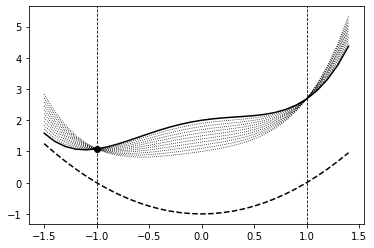
\includegraphics[width=0.5\textwidth]{fig1}
\caption{1 一个对偶可行点的下界}
\end{figure}
      图1用$x\in\mathbf{R}$并且有一个不等式约束的简单问题解释了不等式$g(\lambda, \nu) \leq p^{\star}$中的下界,实线为目标函数$f_{0}$,虚数为约束函数$f_{1}$。可行集合为区间[-1,1]。最优点和最优值为$x^{*}=-1,p^{*}=1.08$。\\
由于在可行集合上对$\lambda\leqslant0\text{ 有 }L(x,\lambda)\leqslant f_{0}(x)$,因此每一个函数$L(x,\lambda)$的最小值都比$p^{*}$小。




\end{frame}

\begin{frame}
	\frametitle{线性方程的最小范数解}
	\begin{equation}
	\begin{array}{ll}
	\text { minimize } & x^{T} x \\
	\text { subject to } & A x=b
    \end{array}
    \end{equation}\\
\onslide<2->{
    \textbf{对偶函数}
    \begin{itemize}[<+->]
    	\item  lagrange函数 为 $L(x, \nu)=x^{T} x+\nu^{T}(A x-b)$
    	\item 为了最小化 $L$, 将梯度设置为零:
    	\begin{equation}
    		\nabla_{x} L(x, \nu)=2 x+A^{T} \nu=0 \quad \Longrightarrow \quad x=-(1 / 2) A^{T}\nu
    	\end{equation}
    	\item 插入$L$ 得到$g$ :
    	\begin{equation}
    		g(\nu)=L\left((-1 / 2) A^{T} \nu, \nu\right)=-\frac{1}{4} \nu^{T} A A^{T} \nu-b^{T} \nu
    	\end{equation}
    	它是一个关于$\nu$的凹二次函数
    \end{itemize}
}
\onslide<4->{
    \textbf{下界性质: }$p^{\star} \geq-(1 / 4) \nu^{T} A A^{T} \nu-b^{T} \nu$ 对于所有 $\nu$
}
\end{frame}
%--------------------------------------------------
\begin{frame}
	\frametitle{标准形式的LP}
	\begin{equation}
	\begin{array}{ll}
	\text{ minimize } & c^{T} x \\
	\text { subject to } & A x=b, \quad x \succeq 0
	\end{array}
    \end{equation}\\
\onslide<2->{
    \textbf{对偶函数}
    \begin{itemize}[<+->]
    	\item lagrange 函数为
    	\begin{equation}
    	\begin{aligned}
    	L(x, \lambda, \nu) &=c^{T} x+\nu^{T}(A x-b)-\lambda^{T} x \\&=-b^{T} \nu+\left(c+A^{T} \nu-\lambda\right)^{T} x
    	\end{aligned}
    	\end{equation}
}
\onslide<3->{
    	\item L 是在$x$上的仿射函数, 因此
    	\begin{equation}
    		g(\lambda, \nu)=\inf _{x} L(x, \lambda, \nu)=\left\{\begin{array}{ll}
    		-b^{T} \nu & A^{T} \nu-\lambda+c=0 \\
    		-\infty & \text { otherwise }
    		\end{array}\right.
    	\end{equation}
    	$g$ 是一条直线,定义域为 $\left\{(\lambda, \nu) \mid A^{T} \nu-\lambda+c=0\right\},$ 因此是凹的
    \end{itemize}
}
\onslide<4->{
    \textbf{下界性质: }$p^{\star} \geq-b^{T} \nu$ if $A^{T} \nu+c \succeq 0$
}
\end{frame}
%---------------------------------------------------
\begin{frame}
	\frametitle{等式约束范数最小化 (Ex.)}
	\begin{equation}
	\begin{array}{ll}
	\text{ minimize } & \|x\| \\
	\text { subject to } & A x=b
	\end{array}
	\end{equation}
\onslide<2->{
	\textbf{对偶函数}
	\begin{equation}
		g(\nu)=\inf _{x}\left(\|x\|-\nu^{T} A x+b^{T} \nu\right)=\left\{\begin{array}{ll}
		b^{T} \nu & \left\|A^{T} \nu\right\|_{*} \leq 1 \\
		-\infty & \text { 其他 }
		\end{array}\right.
	\end{equation}
	其中 $\|v\|_{*}=\sup _{\|u\| \leq 1} u^{T} v$ ,$\|\cdot\|$是对偶范数 \\
}
\onslide<3->{
	
	\textbf{证明:}	
    	\begin{itemize}
\item  
$\inf _{x}\left(\|x\|-y^{T} x\right)= \left\{\begin{array}{cl}
0 & \|y\|_{*} \leq 1\\
-\infty, & \textnormal{否则}\\
\end{array}\right.
$
	  	\item 如果 $\|y\|_{*} \leq 1$, 那么 $\|x\|-y^{T} x \geq 0$ 对于任意 $x,$  如果$x=0$,则相等
		\item 如果 $\|y\|_{*}>1,$ 令 $x=t u$ 其中 $\|u\| \leq 1, u^{T} y=\|y\|_{*}>1$
		\begin{equation}
			\|x\|-y^{T} x=t\left(\|u\|-\|y\|_{*}\right) \rightarrow-\infty \quad \text { 当 } t \rightarrow \infty
		\end{equation}
	\end{itemize}	
 
 \textbf{下界性质:}
    $p^{\star} \geq b^{T} \nu$  如果 $\left\|A^{T} \nu\right\|_{*} \leq 1$
}

\end{frame}
%--------------------------------------------------
\begin{frame}
	\frametitle{双向分区(Two-way partitioning)}
	\begin{equation}
	\begin{array}{ll}
	\text{ minimize } & x^{T} W x \\
	\text { subject to } & x_{i}^{2}=1, \quad i=1, \ldots, n
	\end{array}
	\end{equation}
\onslide<2->{
	\begin{itemize}
		\item 非凸问题;可行集包含$2^n$个离散点
		\item  解释: 将$\{1,\cdots, n\}$ 分成两个集合;
 \hint{$W_{ij}$ 是将$i, j$ 分到相同集合的成本; $-W_{ij}$ 是分配到不同集合的成本}
	\end{itemize}
}
\onslide<3->{
	\textbf{对偶函数}
	\begin{equation}
	\begin{aligned}
    &\begin{aligned}
    g(\nu)=\inf _{x}\left(x^{T} W x+\sum_{i} \nu_{i}\left(x_{i}^{2}-1\right)\right) &=\inf _{x} x^{T}(W+\textbf{diag}(\nu)) x-\mathbf{1}^{T} \nu \\
    &=\left\{\begin{array}{ll}
    -\mathbf{1}^{T} \nu & W+\textbf{diag}(\nu) \succeq 0 \\
    -\infty & \text { 其他 }
    \end{array}\right.
    \end{aligned}
    \end{aligned}
    \end{equation}
}
\onslide<4->{
    \textbf{下界性质: }$p^{\star} \geq-1^{T} \nu \text { 如果} W+\textbf{diag}(\nu) \succeq 0$\\
}
\onslide<5->{
%\begin{example}
 例如: $\nu=-\lambda_{\min }(W) \mathbf{1} \text { gives bound } p^{\star} \geq n \lambda_{\min }(W)$
%\end{example}
}
\end{frame}
%--------------------------------------------------
\begin{frame}
	\frametitle{Lagrange对偶和共轭函数}
	\begin{equation}
	\begin{array}{ll}
	\text{ minimize } & f_{0}(x) \\
	\text { subject to } & A x \preceq b, \quad C x=d
	\end{array}
	\end{equation}\\
\onslide<2->{
	\textbf{对偶函数}
	\begin{equation}
		\begin{aligned}
		g(\lambda, \nu) &=\inf _{x \in \text{dom} f_{0}}\left(f_{0}(x)+\left(A^{T} \lambda+C^{T} \nu\right)^{T} x-b^{T} \lambda-d^{T} \nu\right) \\
		&=-f_{0}^{*}\left(-A^{T} \lambda-C^{T} \nu\right)-b^{T} \lambda-d^{T} \nu
		\end{aligned}
	\end{equation}
	\begin{itemize}[<+->]
		\item 共轭的定义: $f^{*}(y)=\sup _{x \in \text{dom} f}\left(y^{T} x-f(x)\right)$
		\item 如果已知$f_{0}$的共轭,则简化对偶的推导
	\end{itemize}
}	
\onslide<3->{
    \begin{example}[熵最大化]
    \begin{equation}
	f_{0}(x)=\sum_{i=1}^{n} x_{i} \log x_{i}, \quad f_{0}^{*}(y)=\sum_{i=1}^{n} e^{y_{i}-1}
	\end{equation}	
    \end{example}
}
\end{frame}
%---------------------------------------------------
\begin{frame}
	\frametitle{对偶问题}
	\textbf{Lagrange对偶问题}
	\begin{equation} 
 	\text{ max}_{\lambda \succeq 0}  \quad g(\lambda, \nu) 
= 
	 \text{ max}_{\lambda \succeq 0}  \quad \min_{x} L(x,\lambda, \nu) 
	\end{equation}
	\begin{itemize}[<+->]
		\item  Lagrange对偶函数: \dred{找到$p^{\star}$上的最优下界 }   
		\item \hint{对偶问题为凸优化问题;} 最优值记为$d^{\star}$
		\item 如果$\lambda \succeq 0$,则 $(\lambda, \nu) \in \text{dom} g$ ,称$\lambda, \nu$是对偶可行的 
	%	\item 通常通过使隐式约束$(\lambda, \nu) \in \text{dom} g$ 显示来简化
	\end{itemize}

\end{frame}

\begin{frame}
   \frametitle{对偶问题}

    \begin{example}[标准形式LP及其对偶 ]
    \begin{columns}
	    \column{0.5\textwidth}
	    \begin{equation}
	    \begin{array}{ll}
	    \text { minimize } & c^{T} x \\
	    \text { subject to } & A x=b \\
	    & x \succeq 0
	    \end{array}
	    \end{equation}
	    \column{0.5\textwidth}
	    \begin{equation}
	    \begin{array}{ll}
	    \text { minimize } & -b^{T} \nu \\
	    \text { subject to } & A^{T} \nu + c \succeq 0
	    \end{array}
	    \end{equation}	
	\end{columns}
    \end{example}

 \begin{itemize}[<+->]
   \item \hint{假设 $A\in \bbr^{m\times n}$, $m<<n$}
\item 原始问题: $x \in \bbr^n$, 对偶问题 $\nu \in \bbr^m$;
\item   $m<<n$ $\rightarrow$ 对偶规划显著减少了变量个数 
\item \hint{何时考虑对偶规划(来减少变量)?}

  \dred{较少的等式约束:许多变量 $\rightarrow$ 对偶问题  }
 \end{itemize}

\end{frame}

%==============================================================
\subsection{弱对偶和强对偶}
\begin{frame}
	\frametitle{弱对偶和强对偶}
	\textbf{弱对偶:} $d^{\star} \leq p^{\star}$
	\begin{itemize}[<+->]
		\item 总是成立(对于凸和非凸问题)
		\item 可以用来寻找难以解决的问题的最优值下界\\
\onslide<2->{		
		例如,解决SDP(半正定规划)问题
		\begin{equation}
			\begin{array}{ll}
			\text { maximize } & -\mathbf{1}^{T} \nu \\
			\text { subject to } & W+\textbf{diag}(\nu) \succeq 0
			\end{array}
		\end{equation}
		\hint{给出了一个关于双向分配问题的下界 } %P9
}
	\end{itemize}
\onslide<3->{
	\textbf{强对偶:} $d^*=p^*$
	\begin{itemize}[<+->]
		\item 一般不成立
		\item (通常)对于凸问题成立
		\item 在凸问题中保证强对偶的条件称为 \textbf{约束规范}
	\end{itemize}
}
\end{frame}
%---------------------------------------------------
\begin{frame}
	\frametitle{Slater约束条件}

\begin{proposition}
   \begin{itemize}
     \item 以下凸问题
	\begin{equation}
		\begin{array}{ll}
		\text{ minimize } & f_{0}(x) \\
		\text { subject to } & f_{i}(x) \leq 0, \quad i=1, \ldots, m \\
		& A x=b
		\end{array}
	\end{equation}
%is convex;

   \item 	  %这是完全可行的, $i.e.$
	\begin{equation}
		\exists x \in \textbf { int } \mathcal{D}: \quad f_{i}(x)<0, \quad i=1, \ldots, m, \quad A x=b
	\end{equation}
\footnotehint{$\mathcal{D} = \cap_{i=0}^m \textbf{dom}\,f_i(x)$}
   \end{itemize}
$\Longrightarrow$ \hint{ 强对偶性成立.}
\end{proposition}
	
\begin{remark}
  \begin{itemize}%[<+->]
		\item 也保证了达到对偶问题的最优解 (如果 $d^* > -\infty$)

     \item %can be sharpened: $e.g.$, can replace \textbf{int} $\mathcal{D}$ with \textbf{relint} $\mathcal{D}$ (interior relative to affine hull);
\smallhint{
仿射不等式不必与严格不等式同时成立: 如果 $f_1,\cdots, f_k$ 是仿射的, 则在下面条件成立时,强对偶性成立:
$$
\exists x \in \textbf { relint } \mathcal{D}:
\   \hint{f_i(x)\leq0,\ i=1,\cdots,m}, \  f_{i}(x)<0, \ i=k+1, \ldots, m, \  A x=b
 $$	
 }

	\end{itemize}

\end{remark}

\end{frame}
%---------------------------------------------------
\begin{frame}{不等式形式的LP问题}
	\textbf{原问题}
	\begin{equation}
	\begin{array}{ll}
	\text{ minimize } & c^{T} x \\
	\text { subject to } & A x \preceq b
	\end{array}
	\end{equation}
\onslide<2->{
	\textbf{对偶函数}
	\begin{equation}
	g(\lambda)=\inf _{x}\left(\left(c+A^{T} \lambda\right)^{T} x-b^{T} \lambda\right)=\left\{\begin{array}{ll}
	-b^{T} \lambda & A^{T} \lambda+c=0 \\
	-\infty & \text { 其他}
	\end{array}\right.
	\end{equation}
}
\onslide<3->{
	\textbf{对偶问题}
	\begin{equation}
	\begin{array}{ll}
	\text { maximize } & -b^{T} \lambda \\
	\text { subject to } & A^{T} \lambda+c=0, \quad \lambda \succeq 0
	\end{array}
	\end{equation}
	\begin{itemize}[<+->]
		\item 由Slater条件得: 如果对某些$\tilde{x}$,$A \tilde{x} \prec b$ ,则$p^* = d^*$ 
		\item \hint{事实上, $p^* = d^*$ 除非原问题和对偶问题不可行}
	\end{itemize}
}
\end{frame}
%--------------------------------------------------
\begin{frame}
	\frametitle{二次规划问题 (Ex.)}
	\textbf{原问题} (假设 $\left.P \in \mathbf{S}_{++}^{n}\right)$
	\begin{equation}
		\begin{array}{ll}
		\text{ minimize } & x^{T} P x \\
		\text { subject to } & A x \preceq b
		\end{array}
	\end{equation}
\onslide<2->{
	\textbf{对偶函数}
	\begin{equation}
	g(\lambda)=\inf _{x}\left(x^{T} P x+\lambda^{T}(A x-b)\right)=-\frac{1}{4} \lambda^{T} A P^{-1} A^{T} \lambda-b^{T} \lambda
	\end{equation}\\
}
\onslide<3->{
	\textbf{对偶问题}
	\begin{equation}
	\begin{array}{ll}
	\text { maximize } & -(1 / 4) \lambda^{T} A P^{-1} A^{T} \lambda-b^{T} \lambda \\
	\text { subject to } & \lambda \succeq 0
	\end{array}
	\end{equation}
	\begin{itemize}
		\item 由Slatera条件:如果对某些$\tilde{x}$,$A \tilde{x} \prec b$ ,则$p^* = d^*$
		\item 事实上, $p^* = d^*$ 总是成立
	\end{itemize}
}
\end{frame}
%--------------------------------------------------
%\begin{frame}
%	\frametitle{A nonconvex problem with strong duality}
%	\begin{equation}
%		\begin{array}{ll}
%		\text { minimize } & x^{T} A x+2 b^{T} x \\
%		\text { subject to } & x^{T} x \leq 1
%		\end{array}
%	\end{equation}
%	$A \nsucceq 0$, hence nonconvex\\
%\onslide<2->{
%	\textbf{Dual function : }$g(\lambda)=\inf _{x}\left(x^{T}(A+\lambda I) x+2 b^{T} x-\lambda\right)$
%}
%\onslide<3->{	
%	\begin{itemize}
%		\item unbounded below if  $A+\lambda I \nsucceq 0 \text { or if } A+\lambda I \succeq 0 \text { and } b \notin \mathcal{R}(A+\lambda I)$
%		\item minimized by $x=-(A+\lambda I)^{\dagger} b \text { otherwise: } g(\lambda)=-b^{T}(A+\lambda I)^{\dagger} b-\lambda$
%	\end{itemize}
%}
%\onslide<4->{	
%	\textbf{Dual problem} and equivalent SDP:
%	\begin{columns}
%	    \column{0.5\textwidth}
%	    \begin{equation}
%	    \begin{array}{ll}
%	    \text { maximize } & -b^{T}(A+\lambda I)^{\dagger} b-\lambda \\
%	    \text { subject to } & A+\lambda I \succeq 0 \\
%	    & b \in \mathcal{R}(A+\lambda I)
%	    \end{array}
%	    \end{equation}
%}
%\onslide<5->{	
%	    \column{0.5\textwidth}
%	    \begin{equation}
%        \begin{array}{ll}
%        \text { maximize } & -t-\lambda  \\
%        \text { subject to } & {\left[\begin{array}{cc}
%        A+\lambda I & b \\
%        b^{T} & t
%        \end{array}\right] \succeq 0}
%        \end{array}
%        \end{equation}
%	\end{columns}
%}
%\onslide<6->{
%    Strong duality although primal problem is not convex (not easy to show)
%}
%\end{frame}
%===============================================================
%\subsection{geometric interpretation}
%\begin{frame}
%	\frametitle{Geometric interpretation}
%	For simplicity, consider problem with one constraint $f_1(x)\leq 0$\\
%\onslide<2->{	
%	\textbf{Interpretation of dual function:}
%	\begin{equation}
%	g(\lambda)=\inf _{(u, t) \in \mathcal{G}}(t+\lambda u), \quad \text { where } \mathcal{G}=\left\{\left(f_{1}(x), f_{0}(x)\right) \mid x \in \mathcal{D}\right\}
%	\end{equation}
%}
%\onslide<3->{
%	\begin{figure}
%		\centering
%		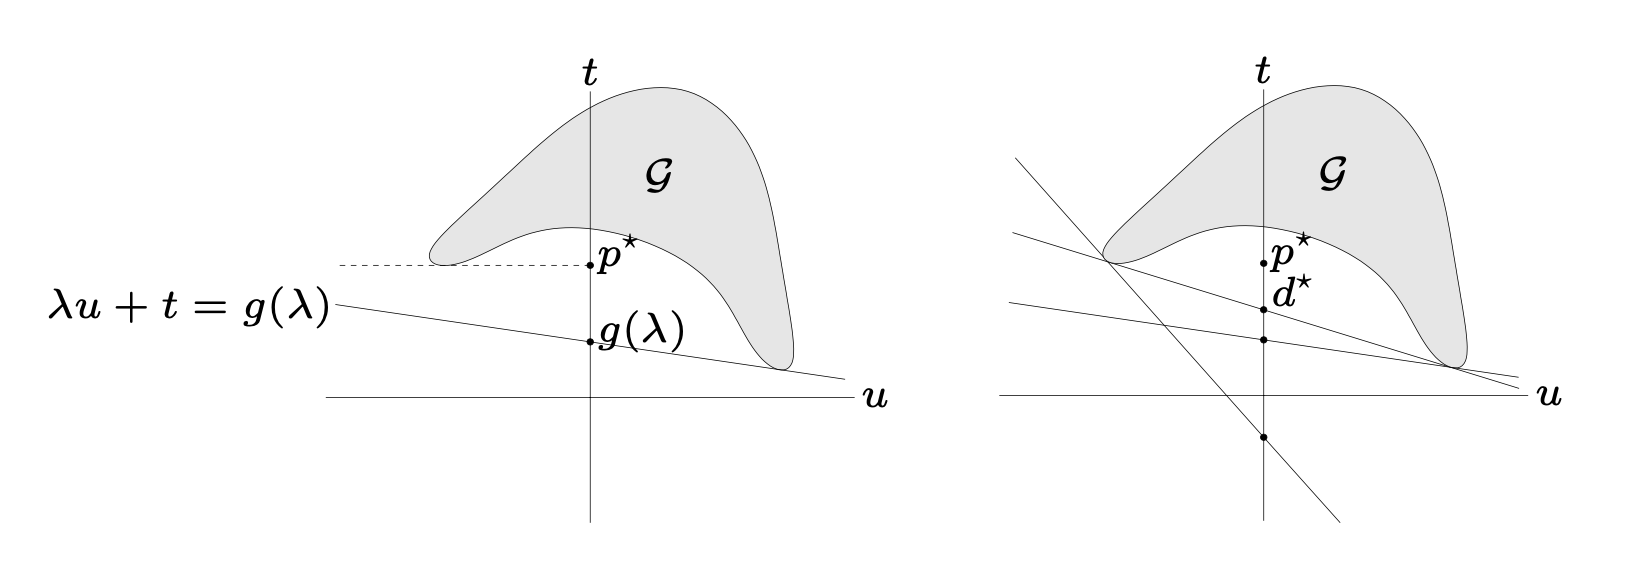
\includegraphics[height=5cm,width=12cm]{Ch5-Geometric-interpretation}	\end{figure}
%}
%\onslide<4->{
%	\begin{itemize}[<+->]
%		\item $\lambda u + t = g(\lambda)$ is (non-vertical) supporting hyperplane to $\mathcal{G}$
%		\item hyperplane intersects $t$-axis at $t = g(\lambda)$
%	\end{itemize}
%}
%\end{frame}
%%---------------------------------------------------
%\subsection{geometric interpretation}
%\begin{frame}
%	\frametitle{Geometric interpretation}
%	\textbf{Epigraph variation:} same interpretation if $\mathcal{G}$ is replaced with
%	\begin{equation}
%	\mathcal{A}=\left\{(u, t) \mid f_{1}(x) \leq u, f_{0}(x) \leq t \text { for some } x \in \mathcal{D}\right\}
%	\end{equation}
%\onslide<2->{
%	\begin{figure}
%		\centering
%		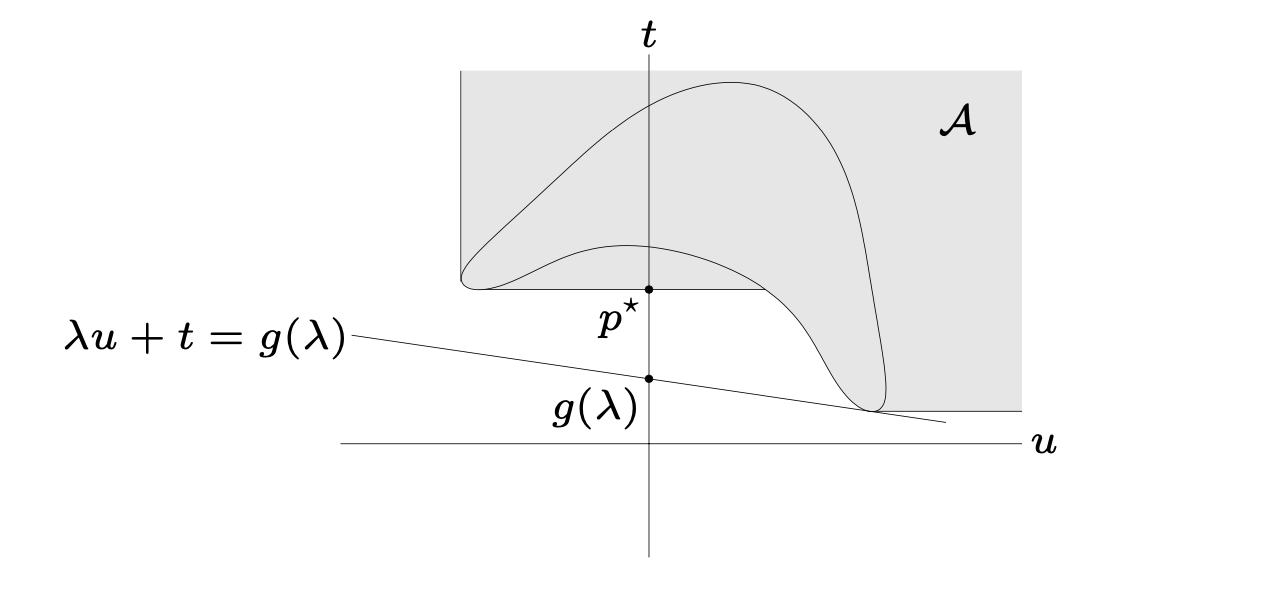
\includegraphics[height=4cm,width=9cm]{Ch5-Geometric-interpretation-2}	\end{figure}
%}
%\onslide<3->{
%	\textbf{Strong duality}
%	\begin{itemize}[<+->]
%		\item holds if there is a non-vertical supporting hyperplane to $\mathcal{A}$ at $(0, p^*)$
%		\item for convex problem, $\mathcal{A}$ is convex, hence has supp. hyperplane at $(0, p^*)$
%		\item Slater's condition: if there exist $(\tilde{u},\tilde{t}) \in \mathcal{A}$ with $\tilde{u} < 0$, then supporting
%		hyperplanes at $(0, p^*)$ must be non-vertical
%	\end{itemize}
%}
%\end{frame}
%==============================================================
\subsection{最优性条件}
\begin{frame}
	\frametitle{互补松弛度}
	\dred{假设强对偶成立,} $x^{\star}$ 是原问题的最优解, $\left(\lambda^{\star}, \nu^{\star}\right)$ 是对偶问题的最优解
\onslide<2->{
	\begin{equation}
		\begin{aligned}
		\dred{f_{0}\left(x^{\star}\right)=g\left(\lambda^{\star}, \nu^{\star}\right) }
&=\inf _{x}\left(f_{0}(x)+\sum_{i=1}^{m} \lambda_{i}^{\star} f_{i}(x)+\sum_{i=1}^{p} \nu_{i}^{\star} h_{i}(x)\right) \\
		& \leq f_{0}\left(x^{\star}\right)+\sum_{i=1}^{m} \lambda_{i}^{\star} f_{i}\left(x^{\star}\right)+\sum_{i=1}^{p} \nu_{i}^{\star} h_{i}\left(x^{\star}\right) \\
		& \leq f_{0}\left(x^{\star}\right)
		\end{aligned}
	\end{equation}\\
}	
\onslide<3->{	
	因此, 这两个不等式取等号
	\begin{itemize}[<+->]
		\item $x^{\star}$ 最小化 $L\left(x, \lambda^{\star}, \nu^{\star}\right)$
		\item $\lambda_{i}^{\star} f_{i}\left(x^{\star}\right)=0$ , $i=1, \ldots, m$ (称为互补松弛):
		\begin{equation}
			\lambda_{i}^{\star}>0 \Longrightarrow f_{i}\left(x^{\star}\right)=0, \quad f_{i}\left(x^{\star}\right)<0 \Longrightarrow \lambda_{i}^{\star}=0
		\end{equation}
	\item $x^*$ 是$L(x,\lambda^*,\nu^*)$的最小值点
	  $\Rightarrow$ $\nabla_{x} L(x,\lambda^*,\nu^*)|_{x=x^*} = 0 $
	\end{itemize}
}
\end{frame}
%--------------------------------------------------
\begin{frame}
	\frametitle{Karush-Kuhn-Tucker (KKT)条件$^{**}$}

	\dred{以下四个条件称为 KKT 条件} (对于可微的 $f_i, h_i$):
	\begin{enumerate}[<+->]
		\item 原始约束: $f_{i}(x) \leq 0, i=1, \ldots, m,\  h_{i}(x)=0, i=1, \ldots, p$\\
		\item 对偶约束: $\lambda \succeq 0$\\
		\item 互补松弛条件: $\lambda_{i} f_{i}(x)=0, i=1, \ldots, m$\\
		\item Lagrange函数在点$x$处的梯度为0 :
	\begin{equation}
		\nabla f_{0}(x)+\sum_{i=1}^{m} \lambda_{i} \nabla f_{i}(x)+\sum_{i=1}^{p} \nu_{i} \nabla h_{i}(x)=0
	\end{equation}
	\end{enumerate}
\onslide<5->{	
%	from page 19
%\hint{Proposition. }
\begin{proposition}
如果强对偶成立,且 $x, \lambda, \nu$ 是原问题和对偶问题的最优解 $\Longrightarrow$  KKT 条件成立.
\end{proposition}
}
\end{frame}
%---------------------------------------------------
\begin{frame}
	\frametitle{凸问题的KKT条件}


\only<1>{
\begin{theorem}

\begin{itemize}

  \item 如果原问题是凸问题: $f_i$ 是凸函数, $h_i$ 是仿射函数
  \item   如果$\tilde{x}, \tilde{\lambda}, \tilde{\nu}$ 满足 $\mathrm{KKT}$条件
\end{itemize}
$\Rightarrow$ $\tilde{x}$, $(\tilde{\lambda}, \tilde{\nu})$ 是零对偶间隙的原始最优解和对偶最优解.
\end{theorem}
\begin{itemize}
\item 注意:
\footnotehint{
  对于任意可微目标和约束函数的\hint{凸} 优化问题, 满足KKT条件的任何点是
原始和对偶最优,并且具有零对偶间隙。 
}
\end{itemize}
}

	
\only<2>{
\textbf{证明:}
	\begin{itemize}
\item $\tilde{x}$: 原始可行解,  $(\tilde{\lambda}, \tilde{\nu})$ 对偶可行解;

\item $\tilde{\lambda}_i \geq 0$     $\Rightarrow$ $L(x,\tilde{\lambda},\tilde{\nu})$ 在$x$处是凸的;

\item 梯度条件: $\nabla_x  L(x,\tilde{\lambda},\tilde{\nu})|_{x=\tilde{x}} = 0$
$\Rightarrow$ $\tilde{x} = \argmin_{x} L(x,\tilde{\lambda},\tilde{\nu})$

\item $$
    \begin{aligned}
      g(\tilde{\lambda},\tilde{\nu}) & = L(\tilde{x},\tilde{\lambda},\tilde{\nu}) \\
        & = f_0(\tilde{x}) + \sum_{i=1}^m \tilde{\lambda}_i f_i(\tilde{x})
            + \sum_{i=1}^p \tilde{\nu}_i h_i(\tilde{x}) \\
          & = f_0(\tilde{x}) \\
    \end{aligned}
$$
%    where
%
%		\item from complementary slackness: $f_{0}(\tilde{x})=L(\tilde{x}, \tilde{\lambda}, \tilde{\nu})$
%		
%		\item from 4th condition (and convexity): $g(\tilde{\lambda}, \tilde{\nu})=L(\tilde{x}, \tilde{\lambda}, \tilde{\nu})$

\item	因此, $f_{0}(\tilde{x})=g(\tilde{\lambda}, \tilde{\nu})$:
零对偶间隙 $\Rightarrow$ $\tilde{x}$, $(\tilde{\lambda}, \tilde{\nu})$ 是原始最优解和对偶最优解。
	\end{itemize}	


}

\only<3->{	

\begin{corollary}
    * 一个具有可微目标函数和约束函数的 \hint{凸} 优化问题


   * 如果满足\textbf{Slater 条件} :
	
$\Rightarrow$ $x$ 和 $(\lambda,\nu)$ 是原始最优解和对偶最优解,当且仅当    	 $(x, \lambda,\nu)$ 满足KKT条件.

\end{corollary}

\bigskip

\begin{footnotesize}
  * Slater条件 $\Rightarrow$ 零对偶间隙,获得对偶最优解;

  * $x$ 是最优解 $\Leftrightarrow$ $\exists (\lambda,\nu)$,和 $x$,
    满足 KKT条件 .

\end{footnotesize}


}
%\only<4->{	
%	\begin{itemize}
%		\item recall that Slater implies strong duality, and dual optimum is attained
%		
%		\item  generalizes optimality condition $\nabla f_0(x) = 0$ for unconstrained problem
%	\end{itemize}
%}

\end{frame}
%---------------------------------------------------
%\begin{frame}
%	\frametitle{KKT conditions for convex problem}
%	\begin{example}[water-filling(assume $\alpha_i > 0$)]
%	\begin{equation}
%	\begin{array}{ll}
%	\text { minimize } & -\sum_{i=1}^{n} \log \left(x_{i}+\alpha_{i}\right) \\
%	\text { subject to } & x \succeq 0, \quad \mathbf{1}^{T} x=1
%	\end{array}
%	\end{equation}
%\onslide<2->{
%	$x$ is optimal iff $x \succeq 0, \mathbf{1}^{T} x=1,$ and there exist $\lambda \in \mathbf{R}^{n}, \nu \in \mathbf{R}$ such that
%	\begin{equation}
%		\lambda \succeq 0, \quad \lambda_{i} x_{i}=0, \quad \frac{1}{x_{i}+\alpha_{i}}+\lambda_{i}=\nu
%	\end{equation}
%}
%\onslide<3->{
%	\begin{itemize}
%		\item if $\nu<1 / \alpha_{i}: \lambda_{i}=0$ and $x_{i}=1 / \nu-\alpha_{i}$
%		\item if $\nu \geq 1 / \alpha_{i}: \lambda_{i}=\nu-1 / \alpha_{i}$ and $x_{i}=0$
%		\item determine $\nu$ from $\mathbf{1}^{T} x=\sum_{i=1}^{n} \max \left\{0,1 / \nu-\alpha_{i}\right\}=1$
%	\end{itemize}
%}
%	\end{example}
%\onslide<4->{
%		\begin{columns}
%	    \column{0.6\textwidth}
%         \textbf{Interpretation}
%	    	 \begin{itemize}
%	     	 \item $n$ patches; level of patch $i$ is at height $\alpha_i$
%	    	\item flood area with unit amount of water
%	    	\item resulting level is $1/\nu^*$
%	    \end{itemize}
%}
%\onslide<5->{
%	    \column{0.5\textwidth}
%	    \begin{figure}
%	    	\centering
%	    	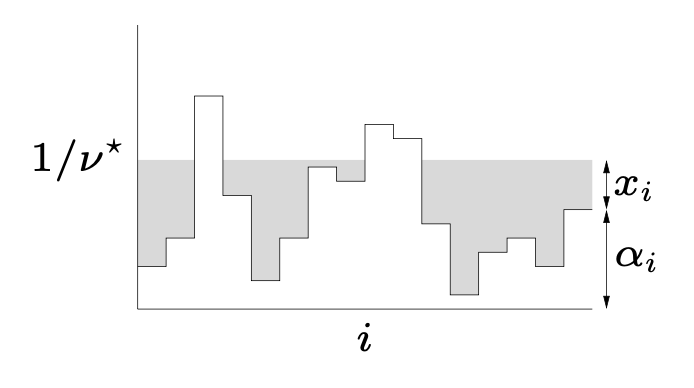
\includegraphics[height=4cm,width=5cm]{Ch5-KKT-conditions-for-convex-problem}
%	    \end{figure}	
%	\end{columns}
%}
%\end{frame}
%==============================================================
%\subsection{perturbation and sensitivity analysis}
%\begin{frame}
%	\frametitle{Perturbation and sensitivity analysis}
%	\textbf{(Unperturbed) optimization problem and its dual}
%	\begin{columns}
%	    \column{0.5\textwidth}
%	    \begin{equation}
%	    \begin{array}{ll}
%	    \text{ minimize } & f_{0}(x) \\
%	    \text { subject to } & f_{i}(x) \leq 0, \quad i=1, \ldots, m \\
%	    & h_{i}(x)=0, \quad i=1, \ldots, p
%	    \end{array}
%	    \end{equation}
%\onslide<2->{
%	    \column{0.5\textwidth}
%	    \begin{equation}
%	    \begin{array}{ll}
%	    \text { maximize } & g(\lambda, \nu) \\
%	    \text { subject to } & \lambda \succeq 0
%	    \end{array}
%	    \end{equation}	
%}
%	\end{columns}
%\onslide<3->{ 	
%    \textbf{Perturbed problem and its dual}
%    \begin{columns}
%    \column{0.5\textwidth}
%     \begin{equation}
%	    \begin{array}{ll}
%	    \text{ min } & f_{0}(x) \\
%	    \text { s.t. } & f_{i}(x) \leq 0, \quad i=1, \ldots, m \\
%	    & h_{i}(x)=0, \quad i=1, \ldots, p
%	    \end{array}
%	    \end{equation}
%}
%\onslide<4->{
%    \column{0.5\textwidth}	
%    \begin{equation}
%        \begin{array}{ll}
%        \max . & g(\lambda, \nu)-u^{T} \lambda-v^{T} \nu \\
%        \text { s.t. } & \lambda \succeq 0
%        \end{array}
%    \end{equation}
%    \end{columns}
%}
%\onslide<5->{
%    \begin{itemize}[<+->]
%    	\item $x$ is primal variable; $u$, $v$ are parameters
%    	\item $p^*(u, v)$ is optimal value as a function of $u$, $v$
%    	\item we are interested in information about $p^*(u, v)$ that we can obtain from the solution of the unperturbed problem and its dual
%    \end{itemize}
% }
%\end{frame}
%%--------------------------------------------------
%\subsection{perturbation and sensitivity analysis}
%\begin{frame}
%	\frametitle{Perturbation and sensitivity analysis}
%	\textbf{Global sensitivity result}\\
%	Assume strong duality holds for unperturbed problem, and that $\lambda$,$\nu$ are dual optimal for unperturbed problem\\
%\onslide<2->{
%	apply weak duality to perturbed problem:
%	\begin{equation}
%        \begin{aligned}
%        p^{\star}(u, v) & \geq g\left(\lambda^{\star}, \nu^{\star}\right)-u^{T} \lambda^{\star}-v^{T} \nu^{\star} \\
%        &=p^{\star}(0,0)-u^{T} \lambda^{\star}-v^{T} \nu^{\star}
%        \end{aligned}
%    \end{equation}\\
%}
%\onslide<3->{
%    \textbf{Sensitivity interpretation}
%    \begin{itemize}[<+->]
%    	\item if $\lambda_i^*$ large: $p^*$ increases greatly if we tighten constraint $i$ ($u_i < 0$)\\
%    \end{itemize}
%}
%\onslide<4->{
%    \begin{itemize}
%    	\item if $\lambda_i^*$ small: $p^*$ does not decrease much if we loosen constraint $i$ ($u_i > 0$)\\
%    \end{itemize}
%}
%\onslide<5->{
%    \begin{itemize}
%    	\item if $\nu_i^*$ large and positive: $p^*$ increases greatly if we take $v_i<0$;\\
%    	      if $\nu_i^*$ large and negative: $p^*$ increases greatly if we take $v_i>0$
%    \end{itemize}
%}
%\onslide<6->{
%    \begin{itemize}
%    	\item if $\nu_i^*$ small and positive: $p^*$ does not decrease much if we take $v_i>0$;\\
%    	      if $\nu_i^*$ small and positive: $p^*$ does not decrease much if we take $v_i<0$
%    \end{itemize}
%}
%\end{frame}
%%--------------------------------------------------
%\subsection{perturbation and sensitivity analysis}
%\begin{frame}
%	\frametitle{Perturbation and sensitivity analysis}
%	\textbf{Local sensitivity: }if (in addition) $p^*(u, v)$ is differentiable at $(0, 0)$, then
%	\begin{equation}
%	    \lambda_{i}^{\star}=-\frac{\partial p^{\star}(0,0)}{\partial u_{i}}, \quad \nu_{i}^{\star}=-\frac{\partial p^{\star}(0,0)}{\partial v_{i}}
%	\end{equation}
%\onslide<2->{
%    \begin{proof}[Proof (for $\lambda_i^*)$]from global sensitivity result,
%    \begin{equation}
%    \begin{array}{l}
%        \frac{\partial p^{\star}(0,0)}{\partial u_{i}}=\lim _{t \searrow 0} \frac{p^{\star}\left(t e_{i}, 0\right)-p^{\star}(0,0)}{t} \geq-\lambda_{i}^{\star} \\
%        \frac{\partial p^{\star}(0,0)}{\partial u_{i}}=\lim _{t \nearrow 0} \frac{p^{\star}\left(t e_{i}, 0\right)-p^{\star}(0,0)}{t} \leq-\lambda_{i}^{\star}
%        \end{array}
%    \end{equation}
%}
%\onslide<3->{
%    hence, equality
%    \begin{columns}
%    \column{0.4\textwidth}
%    $p^*(u)$ for a problem with one (inequality) constraint:
%}
%\onslide<4->{
%    \column{0.5\textwidth}	
%    \begin{figure}
%    	\centering
%    	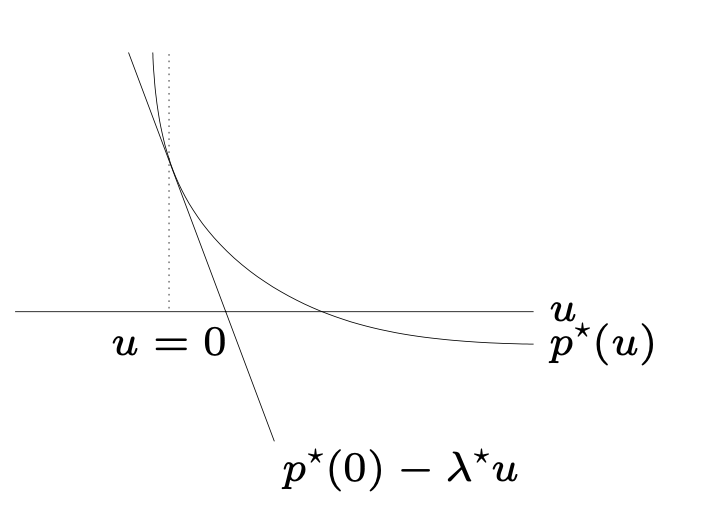
\includegraphics[height=4cm,width=5cm]{Ch5-Perturbation-and-sensitivity-analysis}
%    \end{figure}
%    \end{columns}
%}
%
%    \end{proof}
%\end{frame}
%%--------------------------------------------------
%\begin{frame}
%	\frametitle{Duality and problem reformulations}
%	\begin{itemize}[<+->]
%		\item equivalent formulations of a problem can lead to very different duals
%		\item reformulating the primal problem can be useful when the dual is difficult
%to derive, or uninteresting
%	\end{itemize}
%\onslide<3->{
%	\textbf{Common reformulations}
%	\begin{itemize}[<+->]
%		\item introduce new variables and equality constraints
%		\item make explicit constraints implicit or vice-versa
%		\item transform objective or constraint functions\\
%		$e.g.$, replace $f_0(x)$ by $\phi(f_0(x))$ with $\phi$ convex, increasing
%	\end{itemize}
%}
%\end{frame}
%%=============================================================
%\subsection{examples}
%\begin{frame}
%	\frametitle{Introducing new variables and equality constraints}
%	\begin{equation}
%		\text {minimize} \quad f_{0}(A x+b)
%	\end{equation}
%	\begin{itemize}[<+->]
%		\item dual function is constant: $g=\inf _{x} L(x)=\inf _{x} f_{0}(A x+b)=p^{\star}$
%		\item we have strong duality, but dual is quite useless
%	\end{itemize}
%\onslide<3->{	
%	\textbf{Reformulated problem and its dual}
%	\begin{columns}
%	    \column{0.5\textwidth}
%	    \begin{equation}
%	    \begin{array}{ll}
%	    \text {minimize} & f_{0}(y) \\
%	    \text {subject to} & A x+b-y=0
%	    \end{array}
%	    \end{equation}
%    }
%    \onslide<4->{
%	    \column{0.5\textwidth}
%	    \begin{equation}
%	    \begin{array}{ll}
%	    \text {maximize} & b^{T} \nu-f_{0}^{*}(\nu) \\
%	    \text {subject to} & A^{T} \nu=0
%	    \end{array}
%	    \end{equation}
%	}
%	\end{columns}
%\onslide<5->{
%	Dual function follows from
%	\begin{equation}
%	\begin{aligned}
%	g(\nu) &=\inf _{x, y}\left(f_{0}(y)-\nu^{T} y+\nu^{T} A x+b^{T} \nu\right) \\
%	&=\left\{\begin{array}{ll}
%	-f_{0}^{*}(\nu)+b^{T} \nu & A^{T} \nu=0 \\
%	-\infty & \text { otherwise }
%	\end{array}\right.
%	\end{aligned}
%	\end{equation}
%}
%\end{frame}
%%--------------------------------------------------
%\begin{frame}
%	\frametitle{Introducing new variables and equality constraints}
%	\textbf{Norm approximation problem:} minimize $\|A x-b\|$
%	\begin{equation}
%		\begin{array}{ll}
%			\text{minimize} & \quad\|y\| \\
%			\text{subject to} & y=A x-b
%		\end{array}
%	\end{equation}
%\onslide<2->{
%	can look up conjugate of $\|\cdot\|$, or derive dual directly
%	\begin{equation}
%	\begin{aligned}
%	g(\nu) &=\inf _{x, y}\left(\|y\|+\nu^{T} y-\nu^{T} A x+b^{T} \nu\right) \\
%	&=\left\{\begin{array}{ll}
%	b^{T} \nu+\inf _{y}\left(\|y\|+\nu^{T} y\right) & A^{T} \nu=0 \\
%	-\infty & \text { otherwise }
%	\end{array}\right.\\
%	&=\left\{\begin{array}{ll}
%	b^{T} \nu & A^{T} \nu=0, \quad\|\nu\|_{*} \leq 1 \\
%	-\infty & \text { otherwise }
%	\end{array}\right.
%	\end{aligned}
%	\end{equation}
%	(see page 6)\\
%}
%\onslide<3->{
%	\textbf{Dual of norm approximation problem}
%	\begin{equation}
%	\begin{array}{ll}
%	\text {maximize} & b^{T} \nu \\
%	\text {subject to} & A^{T} \nu=0, \quad\|\nu\|_{*} \leq 1
%	\end{array}
%	\end{equation}
%}
%\end{frame}
%%-------------------------------------------------
%\begin{frame}
%	\frametitle{Implicit constraints}
%	\textbf{LP with box constraints: }primal and dual problem
%\onslide<2->{
%	\begin{columns}
%	    \column{0.5\textwidth}
%	    \begin{equation}
%	    \begin{array}{ll}
%	    \text{minimize} & c^{T} x \\
%	    \text {subject to} & A x=b \\
%	    & -\mathbf{1} \preceq x \preceq \mathbf{1}
%	    \end{array}
%	    \end{equation}
%}
%\onslide<3->{
%	    \column{0.5\textwidth}
%	    \begin{equation}
%	    \begin{array}{cl}
%	    \text {maximize} & -b^{T} \nu-\mathbf{1}^{T} \lambda_{1}-\mathbf{1}^{T} \lambda_{2} \\
%	    \text {subject to} & c+A^{T} \nu+\lambda_{1}-\lambda_{2}=0 \\
%	    & \lambda_{1} \succeq 0, \quad \lambda_{2} \succeq 0
%	    \end{array}
%	    \end{equation}
%	\end{columns}
%}
%\onslide<4->{	
%    \textbf{Reformulation with box constraints made implicit}
%    \begin{equation}
%  	\begin{array}{ll}
%        \text {minimize} & f_{0}(x)=\left\{\begin{array}{ll}
%        c^{T} x & -\mathbf{1} \preceq x \preceq \mathbf{1} \\
%        \infty & \text { otherwise }
%        \end{array}\right. \\
%        \text {subject to} & A x=b
%    \end{array}
%    \end{equation}
%}
%\onslide<5->{
%    dual function
%    \begin{equation}
%    	\begin{aligned}
%    	g(\nu) &=\inf _{-1 \preceq x \preceq 1}\left(c^{T} x+\nu^{T}(A x-b)\right) \\
%    	&=-b^{T} \nu-\left\|A^{T} \nu+c\right\|_{1}
%    	\end{aligned}
%    \end{equation}
%}
%\onslide<6->{
%    \textbf{Dual problem:} maximize $-b^{T} \nu-\left\|A^{T} \nu+c\right\|_{1}$
% }
%\end{frame}
%============================================================
%\subsection{generalized inequalities}
%\begin{frame}
%	\frametitle{Problems with generalized inequalities}
%	\begin{equation}
%	\begin{array}{ll}
%	\text{minimize} & f_{0}(x) \\
%	\text {subject to} & f_{i}(x) \preceq_{K_{i}} 0, \quad i=1, \ldots, m \\
%	& h_{i}(x)=0, \quad i=1, \ldots, p
%	\end{array}
%	\end{equation}
%	$\preceq_{K_i}$is generalized inequality on $\textbf{R}^{k_{i}}$\\
%	
%	\textbf{definitions} are parallel to scalar case:
%	\begin{itemize}
%		\item Lagrange multiplier for $f_{i}(x) \preceq_{K_{i}} 0$ is vector $\lambda_{i} \in \mathbf{R}^{k_{i}}$
%		\item Lagrangian $L: \mathbf{R}^{n} \times \mathbf{R}^{k_{1}} \times \cdots \times \mathbf{R}^{k_{m}} \times \mathbf{R}^{p} \rightarrow \mathbf{R}$, is defined as
%		\begin{equation}
%			L\left(x, \lambda_{1}, \cdots, \lambda_{m}, \nu\right)=f_{0}(x)+\sum_{i=1}^{m} \lambda_{i}^{T} f_{i}(x)+\sum_{i=1}^{p} \nu_{i} h_{i}(x)
%		\end{equation}
%		\item dual function $g: \mathbf{R}^{k_{1}} \times \cdots \times \mathbf{R}^{k_{m}} \times \mathbf{R}^{p} \rightarrow \mathbf{R}$, is defined as
%		\begin{equation}
%			g\left(\lambda_{1}, \ldots, \lambda_{m}, \nu\right)=\inf _{x \in \mathcal{D}} L\left(x, \lambda_{1}, \cdots, \lambda_{m}, \nu\right)
%		\end{equation}
%	\end{itemize}
%\end{frame}
%-------------------------------------------------
%\begin{frame}
%	\frametitle{Problems with generalized inequalities}
%	\textbf{lower bound property:} if $\lambda_{i} \succeq_{K_{i}^{*}} 0,$ then $g\left(\lambda_{1}, \ldots, \lambda_{m}, \nu\right) \leq p^{\star}$\\
%	proof: if $\tilde{x}$ is feasible and $\lambda \succeq_{K_{i}^{*}} 0,$ then
%	\begin{equation}
%		\begin{aligned}
%		f_{0}(\tilde{x}) & \geq f_{0}(\tilde{x})+\sum_{i=1}^{m} \lambda_{i}^{T} f_{i}(\tilde{x})+\sum_{i=1}^{p} \nu_{i} h_{i}(\tilde{x}) \\
%		& \geq \inf _{x \in \mathcal{D}} L\left(x, \lambda_{1}, \ldots, \lambda_{m}, \nu\right) \\
%		&=g\left(\lambda_{1}, \ldots, \lambda_{m}, \nu\right)
%		\end{aligned}
%	\end{equation}
%   minimizing over all feasible $\tilde{x}$ gives $p^{\star} \geq g\left(\lambda_{1}, \ldots, \lambda_{m}, \nu\right)$\\
%    \textbf{dual problem}
%    \begin{equation}
%   	\begin{array}{ll}
%    	\text {maximize} & g\left(\lambda_{1}, \ldots, \lambda_{m}, \nu\right) \\
%    	\text {subject to} & \lambda_{i} \succeq_{K_{i}}^{*} 0, \quad i=1, \ldots, m
%   	\end{array}
%    \end{equation}
%    \begin{itemize}
%    	\item weak duality: $p^{\star} \geq d^{\star}$ always
%   	\item strong duality: $p^{\star}=d^{\star}$ for convex problem with constraint qualification (for example, Slater's: primal problem is strictly feasible)
%    \end{itemize}
%\end{frame}
%---------------------------------------------------
%\begin{frame}
%	\frametitle{Semidefinite program}
%	\textbf{primal SDP }$\left(F_{i}, G \in \mathbf{S}^{k}\right)$\\
%	\begin{equation}
%		\begin{array}{ll}
%			\text{minimize} & \quad c^{T} x\\
%			\text{subject to} & x_{1} F_{1}+\cdots+x_{n} F_{n} \preceq G
%		\end{array}
%	\end{equation}
%	\begin{itemize}
%		\item Lagrange multiplier is matrix $Z \in \mathbf{S}^{k}$
%		\item Lagrangian $L(x, Z)=c^{T} x+\textbf{tr}\left(Z\left(x_{1} F_{1}+\cdots+x_{n} F_{n}-G\right)\right)$
%		\item dual function
%		\begin{equation}
%		g(Z)=\inf _{x} L(x, Z)=\left\{
%		\begin{array}{ll}
%		-\textbf{tr}(G Z) & \textbf{tr}\left(F_{i} Z\right)+c_{i}=0, \quad i=1, \ldots, n \\
%		-\infty & \text {otherwise}
%		\end{array}\right.
%		\end{equation}
%	\end{itemize}
%	\textbf{dual SDP}
%	\begin{equation}
%		\begin{array}{ll}
%		\text {maximize} & -\textbf{tr}(G Z) \\
%		\text {subject to} & Z \succeq 0, \quad \textbf{tr}\left(F_{i} Z\right)+c_{i}=0, \quad i=1, \ldots, n
%		\end{array}
%	\end{equation}
%	$p^{\star}=d^{\star}$ if primal SDP is strictly feasible $\left(\exists x\right.$ with $\left.x_{1} F_{1}+\cdots+x_{n} F_{n} \prec G\right)$
%\end{frame}




\begin{frame}
  \frametitle{应用: 支持向量机}

  \begin{itemize}
    \item 二分类问题
    \item 训练集: $\{x_i,y_i\}_{i=1}^{n}$, $x_i \in \mathbb{R}^d$, $y_i \in \{1,-1\}$

    \item 线性分类器: $y  = \langle w,x\rangle +b$
    
    \item 支持向量机分类 
    $$
       \begin{array}{cl}
         \min_{w,b} & \frac{1}{2}\|w\|^2 \\
         s.t.  & y_i (\langle w,x_i\rangle +b) \geq 1, i=1\cdots,n\\
       \end{array}
      $$ 
      \footnotehint{所有样本均正确分类.}
      
    \item 验证其Lagrange对偶问题: 
    
        $$
       \begin{array}{cl}
         \max_{\alpha} & -\frac{1}{2}\sum_{i=1}^n \sum_{j=1}^n \alpha_i\alpha_j y_iy_j \langle x_i,x_j\rangle + \langle \mathbf{1},\alpha\rangle \\
         s.t.  & \langle \alpha,y\rangle = 0\\
            & \alpha_i \geq 0, \quad i=1,\dots,n\\
       \end{array}
      $$ 
  \end{itemize}

\end{frame}

\begin{frame}
  \frametitle{应用: 支持向量机 (Ex.)}

  \begin{itemize}
     

    \item \hint{软间隔(Soft-margin)} 支持向量机分类
    $$
       \begin{array}{cl}
         \min_{w,b} & \frac{1}{2}\|w\|^2 + C \sum_{i=1}^n \xi_i \\
         s.t.  & y_i (\langle w,x_i\rangle +b) \geq \dred{1 -\xi_i,} i=1\cdots,n\\
       \end{array}
      $$
      \footnotehint{允许一些分类错误的样本.}

    \item 验证其Lagrange对偶问题:

        $$
       \begin{array}{cl}
         \max_{\alpha} & -\frac{1}{2}\sum_{i=1}^n \sum_{j=1}^n \alpha_i\alpha_j y_iy_j \langle x_i,x_j\rangle + \langle \mathbf{1},\alpha\rangle \\
         s.t.  & \langle \alpha,y\rangle = 0\\
            & \dred{C\geq } \alpha_i \geq 0, \quad i=1,\dots,n\\
       \end{array}
      $$
  \end{itemize}

\end{frame}

%\begin{frame}
%  \frametitle{对偶乘子的经济学解释}
%
%    $$
%       \begin{array}{cl}
%         \min_{x} & f_0(x) \\
%         s.t.   
%            & f_i(x)\leq 0, \quad i=1,\dots,m\\
%       \end{array}
%      $$
%
%
%\begin{itemize}
%  \item $x$: 企业如何运作 
%  \item $f_0(x)$:成本;  \qquad $-f_0(x)$: 利润
%  \item $f_i(x) \leq 0$:资源的限制 
%  \item 最优利润: $-p^*$
%  
%\end{itemize}
%
%\end{frame}

%\begin{frame}
%  \frametitle{对偶乘子的经济学解释}
%
%\begin{itemize}
% % \item<1-> 假设:不再严格受资源限制 
%  
%  \item<1-> $\lambda_i\geq 0$: %违反规定的价格 $f_i(x)\leq 0$
%
%         \footnotehint{  以相同价格$\lambda$,公司可出售任何未使用的第$i$种 资源
%          }
% \item<1-> $L(x,\lambda) = f_0(x)  +\sum_{i=1}^m \lambda_i f_i(x)$: 
% 运行条件 $x$的总成本 $=$ 成本 $-$ 资源出售收入 
% 
% \item<2-> 对偶函数 $g(\lambda) \defeq \min_x L(x,\lambda)$:  
%   最优成本 \footnotehint{(约束价格向量 $\lambda$的函数)}
%          
%\item<2-> 对偶目标值 $d^* = \max_{\lambda} g(\lambda)$:
%  最优价格下的最优成本 
%  
% \item<2-> $d^*\leq p^*$: 
% 
% $x^*$: 原始最优解 $\Rightarrow$          
%    $L(x^*,\lambda)\leq f_0(x^*), \forall \lambda \geq 0$
%    
%  \item<3-> $p^*  -d^*$ (对偶间隙) :允许企业为违反约束支付费用(并接受非关税约束费用)的最低限制
%  \item<3-> $p^*-d^* = 0$ (强对偶性):$\exists$ 对偶最优解 $\lambda^*$: 对公司没有好处
%  
%  \item<3-> $\lambda^*$ (对偶最优向量 ): 
%  
%  对于原始问题的一个 \hint{影子价格} 
%\end{itemize}
%
%\end{frame}



\begin{frame}[allowframebreaks]
  \frametitle{作业}
  
  \begin{enumerate}
  	   \item   考虑如下优化问题
    \begin{equation}
		\begin{array}{ll}
		\text{ minimize }& x^{2}-2x+1\\
		\text { subject to }& (x-1)(x-5)\leqslant0
		\end{array}
	\end{equation}
 其中${\mathbf{x}\in\mathbf{R}^{n}}$\\
(1)分析原问题,给出可行集、最优值以及最优解\\
(2)画出目标函数关于$x$的图像,并在图像上画出可行集、最优值以及最优解。画出${\lambda}$=0.2时,Lagrange函数${L(x,\lambda)}$关于$x$的图像,验证下界性质:${p^*\geqslant\inf_xL(x,\lambda)}$对${\lambda\geqslant0}$成立。推导并画出Lagrange对偶函数$g$.
  	\item 考虑如下凸分段线性函数最小化问题	
   \begin{equation}
		\begin{array}{ll}
		\text{ minimize }&\max_{i=1,\ldots,m}(a_i^\mathrm{T}\boldsymbol{x}+b_i)\\
		\end{array}
	\end{equation}
     其中${\mathbf{x}\in\mathbf{R}^{n}}$\\
(1)考虑等式问题
\begin{equation}
		\begin{array}{ll}
		\text{ minimize }& \max_{i=1,\cdots,m}y_i\\
		\text { subject to }& \boldsymbol{a}_{i}^{\mathrm{T}}\boldsymbol{x}+b_{i}=y_{i},i=1,\cdots,m
		\end{array}
	     \end{equation} 
其中${\mathbf{x}\in\mathbf{R}^{n}}$,${\mathbf{y}\in\mathbf{R}^{m}}$,推导出Lagrange对偶问题。\\

(2)将分段线性问题(34)表述为LP问题并写出LP问题的对偶问题。将LP对偶与(1)中所求得的对偶问题联系起来。 
  	
  	\item 
设有若干二分类问题的观测样本${\{(x_i,y_i)\}_{i=1}^\mathrm{n}\subseteq\mathbf{R}^d\times\{+1,-1\}}$,考虑线性支持向量机模型:\\
\begin{equation}
	min_{w\in\mathbf{R}^{4},b\in\mathbf{R}}\frac{1}{2}\|\boldsymbol{w}\|^{2}+C\sum_{i=1}^{n}l(x_{i},y_{i};\boldsymbol{w},b)
	\end{equation}\\
  ${\mathrm{c}>0}$为参数,${l(x_i,y_i;\boldsymbol{w},b)=\max(0,1-y_i(\boldsymbol{w}^\top x_i+b))}$为样本点${(x_{i},y_{i})}$的经验损失,对应Hinge损失函数${l(t)=\max(0,1-t)}$,函数${y(x)=w^{\top}x+b}$为判别函数。\\
(1)将线性支持向量机模型化为凸二次规划模型,并写出该规划模型的对偶问题。\\
(2)结合凸二次规划模型的最优化条件,说明哪些样本对模型起作用,哪些不起作用。

  	\item 通过引入新变量${y_{i}\in\mathbf{R}^{m_{i}}}$以及等式约束${y_{i}=A_{i}x+b_{i}}$,推导出下式的对偶问题\\
     \begin{equation}
	\mathrm{minimize}\quad\sum_{i=1}^N\left\|A_ix+b_i\right\|_2
	\end{equation}
  其中${A_{i}\in\mathbf{R}^{m_{i}\times n}}$,${b_{i}\in\mathbf{R}^{m_{i}}}$

\item 考虑Lasso模型
\begin{equation}
	\begin{array}{ll}\\
\text{minimize}&\left\|Ax+b\right\|^2+\lambda\cdot\left|x\right|_1\
     \end{array}
	\end{equation}
其中${A\in\mathbf{R}^{m\times n},\boldsymbol{b}\in\mathbf{R}^{m},\lambda>0}$,假设模型有唯一解,证明该模型的最优解关于${\lambda}$是分片线性的。
\item 考虑QCQP问题
           \begin{equation}
		\begin{array}{ll}
		\text{ minimize }& \frac{1}{2}(x_1^2+x_2^2)-4\\
		\text { subject to }& (x_{1}-1)^{2}+(x_{2}-1)^{2}\leqslant4
		\end{array}
	     \end{equation} 
其中变量${x\in\mathbb{R}^{2}}$\\
(1)写出最优点${x^{*}}$和最优值${p^{*}}$。\\
(2)写出KKT条件。\\
(3)求解Lagrange对偶问题并说明强对偶性性是否成立。
\item 推导出下面问题的KKT条件
           \begin{equation}
		\begin{array}{ll}
		\text{ minimize }& \operatorname{tr}X-\log\det X\\
		\text { subject to }& X\boldsymbol{s}=\boldsymbol{y}
		\end{array}
	     \end{equation} 
其中${X\in\mathbf{S}^{n}}$,定义域${\mathbf{s}_{++}^{n}}$。已知${y\in\mathbf{R}^{n},s\in\mathbf{R}^{n}}$且${s^{\mathrm{T}}y=1}$,证明最优解为
          \begin{equation}
X^{^{*}}=I+yy^{\mathrm{T}}-\frac{1}{s^{\mathrm{T}}s}ss^{\mathrm{T}}
          \end{equation}
\end{enumerate}
\end{frame}


\end{document}

